\documentclass{article}
\usepackage{tikz}
\usepackage{float}
\usepackage{enumerate}
\usepackage{amsmath}
\usepackage{amsthm}
\usepackage{bm}
\usepackage{indentfirst}
\usepackage{siunitx}
\usepackage[utf8]{inputenc}
\usepackage{graphicx}
\graphicspath{ {Images/} }
\usepackage{float}
\usepackage{mhchem}
\usepackage{chemfig}
\allowdisplaybreaks

\title{6.041 Problem Set 5}
\author{Robert Durfee - R02}
\date{October 11, 2018}

\begin{document}

\maketitle

\section*{Problem 1}

\textit{For each one of the following figures, identify if it corresponds to
a valid CDF. The value of the CDF at points of discontinuity is indicated
with a small solid circle.}

\subsection*{Part A}

\begin{center}
    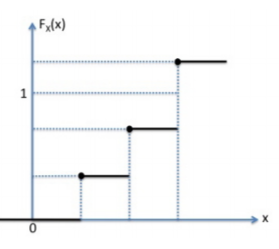
\includegraphics[scale=1]{Images/P1A.PNG}
\end{center}

This figure cannot correspond to a legitimate CDF as its maximum value is
greater than 1.

\subsection*{Part B}

\begin{center}
    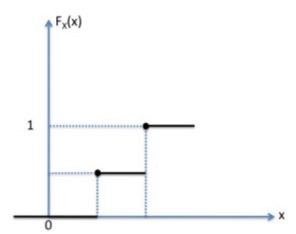
\includegraphics[scale=1]{Images/P1B.PNG}
\end{center}

This is a valid CDF.

\subsection*{Part C}

\begin{center}
    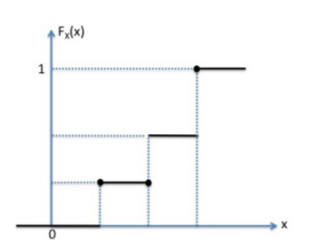
\includegraphics[scale=1]{Images/P1C.PNG}
\end{center}

This is not be a valid CDF because of the value of the second discontinuity.

\subsection*{Part D}

\begin{center}
    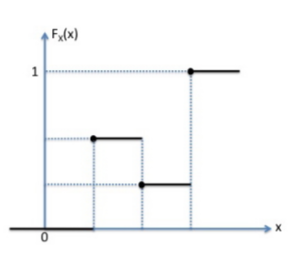
\includegraphics[scale=1]{Images/P1D.PNG}
\end{center}

This cannot be a valid CDF because it isn't monotonically increasing.

\section*{Problem 2}

\textit{Random variables $ X $ and $ Y $ are distributed according to the
joint PDF}
$$ f_{X,Y}(x, y) = \begin{cases}
    ax & \mathrm{if} \, 1 \leq x \leq 2 \, \mathrm{and} \, 0 \leq y \leq x \\
    0 & \mathrm{otherwise}
\end{cases} $$

\subsection*{Part A}

\textit{Find the constant $ a $.}

\bigbreak

From the axiom of normalization, 
$$ 1 = \iint f_{X,Y}(x, y) dx dy $$
Applying the limits of integration
\begin{align*}
    1 &= \int\limits_1^2 \int\limits_0^x a x dy dx \\
      &= a \int\limits_1^2 x \int\limits_0^x dy dx \\
      &= a \int\limits_1^2 x \left( y \right)_0^x dx \\
      &= a \int\limits_1^2 x \left( x - 0 \right) dx \\
      &= a \int\limits_1^2 x^2 dx \\
      &= a \left( \frac{x^3}{3} \right)_1^2 \\
      &= a \left( \frac{2^3}{3} - \frac{1^3}{3} \right) \\
      &= a \left( \frac{8 - 1}{3} \right) \\
      &= \frac{7 a}{3}
\end{align*}
Therefore, $ a = 3 / 7 $.

\subsection*{Part B}

\textit{Determine the marginal PDF $ f_Y(y) $.}

\bigbreak

The joint PDF applies for the region $ 1 \leq x \leq 2,\, 0 \leq y \leq x $.
This is the same as the combination of two regions $ y \leq x \leq 2,\, 1
\leq y \leq 2 $ and $ 1 \leq x \leq 2,\, 0 \leq y \leq 0 $. Integrating over
both of these regions with respect to $x$ will give the marginal PDF of $Y$.
$$ f_Y(y) = \begin{cases}
    \int\limits_y^2 f_{X,Y}(x, y) dx & 1 \leq y \leq 2 \\
    \int\limits_1^2 f_{X,Y}(x, y) dx & 0 \leq y \leq 1 \\
    0 & \mathrm{otherwise}
\end{cases} $$
Applying the integration in the first case
\begin{align*}
    \int\limits_y^2 f_{X,Y}(x, y) dx &= \int\limits_y^2 \frac{3}{7} x dx \\
    &= \frac{3}{7} \int\limits_y^2 x dx \\
    &= \frac{3}{7} \left( \frac{x^2}{2} \right)_y^2 \\
    &= \frac{3}{7} \left( \frac{2^2}{2} - \frac{y^2}{2} \right) \\
    &= \frac{3}{7} \left( \frac{4 - y^2}{2} \right) \\
    &= \frac{12 - 3 y^2}{14}
\end{align*}
Applying the integration in the second case
\begin{align*}
    \int\limits_1^2 f_{X,Y}(x, y) dx &= \int\limits_1^2 \frac{3}{7} x dx \\
    &= \frac{3}{7} \int\limits_1^2 x dx \\
    &= \frac{3}{7} \left( \frac{2^2}{2} - \frac{1^2}{2} \right) \\
    &= \frac{3}{7} \left( \frac{4 - 1}{2} \right) \\
    &= \frac{9}{14}
\end{align*}
Therefore, the marginal PDF of $Y$ is
$$ f_Y(y) = \begin{cases}
    \left( 12 - 3 y^2 \right) / 14 & 1 \leq y \leq 2 \\
    9 / 14 & 0 \leq y \leq 1 \\
    0 & \mathrm{otherwise}
\end{cases} $$

\section*{Problem 3}

\textit{Paul is vacationing in Monte Carlo. On any given night, he takes X
dollars to the casino and returns with Y dollars. The random variable X has
the PDF shown in the figure. Conditional on X = x, the continuous random
variable Y is uniformly distributed between zero and 2x.}

\begin{center}
    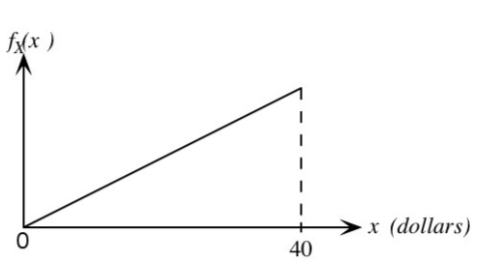
\includegraphics[scale=1]{Images/P3.PNG}
\end{center}

\subsection*{Part A}

\textit{Determine the joint PDF $ f_{X,Y}(x, y) $.}

\bigbreak

From the diagram, the PDF for $X$ must be linear through the origin. Since $
0 \leq x \leq 40 $, the slope of the line is given through the normalization
axiom
\begin{align*}
    1 &= \int\limits_0^{40} c x dx \\
    &= c \int\limits_9^{40} x dx \\
    &= c \left( \frac{x^2}{2} \right)_0^{40} \\
    &= c \left( \frac{40^2}{2} - \frac{0^2}{2} \right) \\
    &= 800 c
\end{align*}
From this, $ c = 1/800 $.
Therefore, the PDF for $X$ is 
$$ f_X(x) = \begin{cases}
    x / 800 & 0 \leq x \leq 40 \\
    0 & \mathrm{otherwise}
\end{cases} $$

Now, the conditional PDF for $Y$ is uniform, therefore it can be written
$$ f_{Y|X}(y \mid x) = \begin{cases}
    1 / 2x & 0 \leq y \leq 2x \\
    0 & \mathrm{otherwise}
\end{cases} $$

From the multiplication rule
$$ f_{X,Y} (x, y) = f_X(x) f_{Y|X}(y \mid x) $$
Therefore, substituting PDFs from above,
$$ f_{X,Y} (x, y) = \begin{cases}
    1 / 1600 & 0 \leq x \leq 40,\, 0 \leq y \leq 2x \\
    0 & \mathrm{otherwise}
\end{cases} $$

\subsection*{Part B}

\textit{On any particular night, Paul makes a profit of $ Z = Y - X $ dollars.
Find the probability that Paul makes a positive profit (i.e., $ P(Z > 0)$). }

\bigbreak

The probability of a positive profit is equivalent to the following
$$ P(Z > 0) = P(Y - X > 0) = P(Y > X) $$
From the last probability, the positive profit is given by the integration of
the joint PDF over the region such that $ y > x $
\begin{align*}
    P(Z > 0) &= \int\limits_0^{40} \int\limits_x^{2x} f_{X,Y}(x, y) dy dx \\
    &= \int\limits_0^{40} \int\limits_x^{2x} \frac{1}{1600} dy dx \\
    &= \frac{1}{1600} \int\limits_0^{40} \left( y \right)_x^{2x} dx \\
    &= \frac{1}{1600} \int\limits_0^{40} \left( 2x - x \right) dx \\
    &= \frac{1}{1600} \int\limits_0^{40} x dx \\
    &= \frac{1}{1600} \left( \frac{x^2}{2} \right)_0^{40} \\
    &= \frac{1}{1600} \left( \frac{40^2}{2} - \frac{0}{2} \right) \\
    &= \frac{1}{1600} \cdot \frac{1600}{2} \\
    &= \frac{1}{2}
\end{align*}
Therefore, the probability of a positive profit is $ P(Z > 0) = 1/2 $.

\subsection*{Part C}

\textit{Find the PDF of Z. Express your answers in terms of z.}

\bigbreak

If $X$ is given, then the profit $Z$ ranges directly with the range of $Y$.
Therefore, maximum profit given $X$ is $2X - X$ and minimum profit given $X$
is $0 - X$. Since each value of $Y$ is of uniform probability given $X$, the
PDF of $Z$ is also uniform given $X$
$$ f_{Z|X}(z \mid x) = \begin{cases}
    1 / 2x & -x \leq z \leq x \\
    0 & \mathrm{otherwise}
\end{cases} $$
From the relationship to marginal PDF
$$ f_Z(z) = \int\limits_{-\infty}^\infty f_X(x) f_{Z|X}(z \mid x) dx $$
The marginal PDF of $Z$ becomes
\begin{align*} f_Z(z) &= \int\limits_0^{40} \frac{x}{1600} \cdot \frac{1}{2x} dx \\
    &= \frac{1}{3200} \int\limits_0^{40} dx \\
    &= \frac{1}{3200} \left(x \right)_0^40 \\
    &= \frac{1}{3200} \left(40 - 0 \right) \\
    &= \frac{1}{80}
\end{align*}
Therefore, the marginal PDF of $Z$ is
$$ f_Z(z) = \begin{cases}
    1/80 & -40 \leq z \leq 40 \\
    0 & \mathrm{otherwise}
\end{cases} $$

\subsection*{Part D}

\textit{Calculate the expected value of Z.}

\bigbreak

Since $Z$ is uniformly distributed over the range $ -40 \leq z \leq 40 $, the
expected value is simply the center of the region which is zero. Therefore,
Paul's expected profit is zero.

\section*{Problem 4}

\textit{The figure below describes the joint PDF of random variables X and Y
. These random variables take values in $[0, 2]$ and $[0, 1]$, respectively.
At $x = 1$, the value of the joint PDF is $1/2$}

\begin{center}
    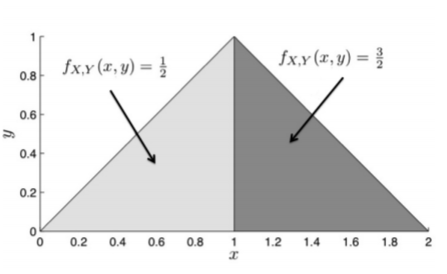
\includegraphics[scale=1]{Images/P4.PNG}
\end{center}

\subsection*{Part A}

\textit{Are X and Y independent?}

\bigbreak

In order for $X$ and $Y$ to be independent, the following must be true
$$ f_{X,Y}(x,y) = f_X(x) f_Y(y) $$
First, determining the equation for the joint PDF given in the graph
$$ f_{X,Y}(x,y) = \begin{cases}
    1/2 & y \leq x \leq 1,\, 0 \leq y \leq 1 \\
    3/2 & 1 < x \leq (2 - y),\, 0 \leq y \leq 1 \\
    0 & \mathrm{otherwise}
\end{cases} $$

To find the marginal PDF for $X$, integrate over all possible $Y$ in the
joint PDF
$$ f_X(x) = \begin{cases}
    \int\limits_0^{x} \frac{1}{2} dy & 0 \leq x \leq 1 \\
    \int\limits_0^{2 - x} \frac{3}{2} dy & 1 < x \leq 2 \\
    0 & \mathrm{otherwise}
\end{cases} $$
Computing the first integral
\begin{align*}
    \int\limits_0^x \frac{1}{2} dy &= \frac{1}{2} \int\limits_0^x dy \\
    &= \frac{1}{2} \left( y \right)_0^x \\
    &= \frac{1}{2} \left( x - 0 \right) \\
    &= \frac{x}{2}
\end{align*}
Computing the second integral
\begin{align*}
    \int\limits_0^{2 - x} \frac{3}{2} dy &= \frac{3}{2} \int\limits_0^{2 - x} dy \\
    &= \frac{3}{2} \left( y \right)_0^{2 - x} \\
    &= \frac{3}{2} \left(2 - x - 0 \right) \\
    &= 3 - \frac{3x}{2}
\end{align*}
Therefore, the marginal PDF for $X$ is
$$ f_X(x) = \begin{cases}
    x / 2 & 0 \leq x \leq 1 \\
    3 - 3x / 2 & 1 < x \leq 2 \\
    0 & \mathrm{otherwise}
\end{cases} $$

To find the marginal PDF of $Y$, integrate over all possible $X$ in the joint
PDF
$$ f_Y(y) = \begin{cases}
    \int\limits_y^1 \frac{1}{2} dx + \int\limits_1^{2 - y} \frac{3}{2} dx & 0 \leq y \leq 1 \\
    0 & \mathrm{otherwise}
\end{cases} $$
Computing the first integral
\begin{align*}
    \int\limits_y^1 \frac{1}{2} dx &= \frac{1}{2} \int\limits_y^1 dx \\
    &= \frac{1}{2} \left( x \right)_y^1 \\
    &= \frac{1}{2} \left( 1 - y \right) \\
    &= \frac{1 - y}{2}
\end{align*}
Computing the second integral
\begin{align*}
    \int\limits_1^{2-y} \frac{3}{2} dx &= \frac{3}{2} \int\limits_1^{2-y} dx \\
    &= \frac{3}{2} \left( x \right)_1^{2-y} \\
    &= \frac{3}{2} \left( 2 - y - 1 \right) \\
    &= \frac{3 (1 - y)}{2}
\end{align*}
Therefore, the marginal PDF for $Y$ is
$$ f_Y(y) = \begin{cases}
    2 - 2y & 0 \leq y \leq 1 \\
    0 & \mathrm{otherwise}
\end{cases} $$

Checking if these are independent, let $X = 1.2$ and $Y = 0.2$,
$$ \frac{3}{2} \neq \left(3 - \frac{3 \cdot 1.2}{2}\right) \cdot \left(2 - 2
\cdot 0.2 \right) $$
Therefore, these two are not independent.

\subsection*{Part B}

\textit{Find $ f_X(x) $. Express your answers in terms of x.}

\bigbreak

As computed above, the marginal PDF for $X$ is
$$ f_X(x) = \begin{cases}
    x / 2 & 0 \leq x \leq 1 \\
    3 - 3x / 2 & 1 < x \leq 2 \\
    0 & \mathrm{otherwise}
\end{cases} $$

\subsection*{Part C}

\textit{Find $ f_{Y|X}(y \mid 0.5) $.}

\bigbreak

From the definition of conditional probability
$$ f_{Y|X}(y \mid x) = \frac{f_{X,Y}(x,y)}{f_X(x)} $$
From the computations above,
$$ f_{Y|X}(y \mid x) = \frac{\begin{cases}
    1/2 & y \leq x \leq 1,\, 0 \leq y \leq 1 \\
    3/2 & 1 < x \leq (2 - y),\, 0 \leq y \leq 1 \\
    0 & \mathrm{otherwise}
\end{cases}}{\begin{cases}
    x / 2 & 0 \leq x \leq 1 \\
    3 - 3x / 2 & 1 < x \leq 2 \\
    0 & \mathrm{otherwise}
\end{cases}} $$
Since $X = 0.5$, this drastically simplifies to
$$ f_{Y|X}(y \mid x) = \frac{1/2}{x/2} $$
Therefore, the conditional PDF is given
$$ f_{Y|X}(y \mid 0.5) = \begin{cases}
    2 & 0 \leq y \leq 0.5 \\
    0 & \mathrm{otherwise}
\end{cases} $$

\subsection*{Part D}

\textit{Find $ f_{X|Y}(x \mid 0.5) $.}

\bigbreak

From the definition of conditional probability
$$ f_{X|Y}(x \mid y) = \frac{f_{X,Y}(x,y)}{f_Y(y)} $$
From the computations above,
$$ f_{X|Y}(x \mid y) = \frac{\begin{cases}
    1/2 & y \leq x \leq 1,\, 0 \leq y \leq 1 \\
    3/2 & 1 < x \leq (2 - y),\, 0 \leq y \leq 1 \\
    0 & \mathrm{otherwise}
\end{cases}}{\begin{cases}
    2 - 2y & 0 \leq y \leq 1 \\
    0 & \mathrm{otherwise}
\end{cases}} $$
Since $Y = 0.5$, this simplifies a little to
$$ f_{X|Y}(x \mid y) = \frac{\begin{cases}
    1/2 & y \leq x \leq 1 \\
    3/2 & 1 < x \leq (2 - y)
\end{cases}}{2 - 2y} $$
Therefore, the conditional PDF is given
$$ f_{X|Y}(x \mid 0.5) = \begin{cases}
    1/2 & 0.5 \leq x \leq 1 \\
    3/2 & 1 < x \leq 1.5 \\
    0 & \mathrm{otherwise}
\end{cases} $$

\subsection*{Part E}

\textit{Let $ R = XY $ and let $A$ be the event $ \{ X < 0.5 \} $. Evaluate $
E[R \mid A] $.}

\bigbreak

From the expected value rule,
$$ E[g(X,Y) \mid A] = \int\limits_{-\infty}^{\infty} g(x, y) f_{X,Y|A}(x, y)
dx $$
The joint PDF from above
$$ f_{X,Y}(x,y) = \begin{cases}
    1/2 & y \leq x \leq 1,\, 0 \leq y \leq 1 \\
    3/2 & 1 < x \leq (2 - y),\, 0 \leq y \leq 1 \\
    0 & \mathrm{otherwise}
\end{cases} $$
From the definition of a conditional PDF given an event
$$ f_{X,Y|A}(x) = \frac{f_{X,Y}(x,y)}{P(A)} $$
The probability of event $A$, $ X < 0.5 $ is given by the joint PDF
\begin{align*}
    \int\limits_0^{0.5}\int\limits_y^{0.5} f_{X,Y}(x,y) dx dy &= \int\limits_0^{0.5}\int\limits_y^{0.5} \frac{1}{2} dx dy \\
    &= \frac{1}{2} \int\limits_0^{0.5} \int\limits_y^{0.5} dx dy \\
    &= \frac{1}{2} \int\limits_0^{0.5} \left(x \right)_y^{0.5} dy \\
    &= \frac{1}{2} \int\limits_0^{0.5} \left(0.5 - y \right) dy \\
    &= \frac{1}{2} \left(0.5 - \frac{y^2}{2} \right)_0^{0.5} \\
    &= \frac{1}{2} \left(\left(0.5 - \frac{0.5^2}{2}\right) - \left(0.5 - \frac{0^2}{2}\right) \right) \\
    &= \frac{1}{16}
\end{align*}
Therefore, the conditional joint PDF is 
$$ f_{X,Y|A}(x) = \begin{cases}
    8 & y \leq x \leq 0.5,\, 0 \leq y \leq 0.5 \\
    0 & \mathrm{otherwise}
\end{cases} $$
Substituting back into the expected value rule
\begin{align*}
    E[X \cdot Y \mid A] &= \int\limits_{0}^{0.5}\int\limits_y^{0.5} 8 x y dx dy \\
    &= 8 \int\limits_0^{0.5} y \int\limits_y^{0.5} x dx dy \\
    &= 8 \int\limits_0^{0.5} y \left(\frac{x^2}{2} \right)_y^{0.5} dy \\
    &= 8 \int\limits_0^{0.5} y \left(\frac{0.5^2}{2} - \frac{y^2}{2} \right) dy \\
    &= 8 \int\limits_0^{0.5} \frac{0.25 y}{2} - \frac{y^3}{2} dy \\
    &= 8 \left(\frac{0.25 y^2}{4} - \frac{y^4}{8} \right)_0^{0.5} \\
    &= 8 \left(\frac{0.25 \cdot 0.5^2}{4} - \frac{0.5^4}{8} \right) \\
    &= \frac{1}{16}
\end{align*}
Therefore, $ E[X\cdot Y \mid X < 0.5] = 1 / 16 $.

\section*{Problem 5}

\subsection*{Part A}

\textit{Let X be a random variable that takes values between 0 and c, for
some $ c > 0 $, so that $P(0 \leq X \leq c) = 1$. Prove that $\mathrm{var}(X)
\leq c^2/4$.}

\bigbreak

From the properties of variance, the following are equivalent
$$ \mathrm{var}(X) = \mathrm{var}(X - c / 2) $$
Since $ 0 \leq X \leq c $, then
$$ -\frac{c}{2} \leq X - \frac{c}{2} \leq \frac{c}{2} $$
Therefore it is easy to see that
$$ E[(X - c/2)^2] \leq \frac{c^2}{4} $$
From the definition of variance
$$ \mathrm{var}(X - c / 2) = E[(X - c/2)^2] - (E[X - c / 2])^2 $$
The first term has to be less than or equal to $ c^2 / 4 $ and the second
term is always non-negative. Therefore
$$ \mathrm{var}(X - c / 2) \leq \frac{c^2}{4} $$
Using, again, the properties of variance, this is equivalent to
$$ \mathrm{var}(X) \leq \frac{c^2}{4} $$

\subsection*{Part B}

\textit{Let X be a non-negative continuous random variable. Using the
definition $E[X] = \int_0^{\infty} x f_X(x) dx $, show that $ E[X] =
\int_0^{\infty} P(X > t) dt $.}

\bigbreak

From the definition of expected value of positive continuous random variables
$$ E[X] = \int\limits_0^\infty x f_X(x) dx $$
However, the relationship between PDF and CDF is as follows
$$ \frac{dF_X(x)}{dx} = f_X(x) $$
Therefore, this definition can be written also as
$$ E[X] = \int\limits_0^\infty x dF_X(x) $$
Thinking in terms of Riemann integrals, this is the same as taking the sum of
horizontal rectangles of height $ dF_X(x) $ and length $x$. But, since the
range of integration is positive and $F_X(x)$ approaches $1$ as $x$ approaches
infinity, this integral can be written as
$$ E[X] = \int\limits_0^\infty 1 - F_X(x) dx $$
Which simply takes vertical rectangles from $F_X(x)$ to $1$ with width $dx$.
This is the same area of integration as above.

Now, from the definition of CDF
$$ F_X(x) = P(X \leq x) $$
For positive random variables, the following must also be true
$$ F_X(x) = 1 - P(X > x) $$
Therefore, the integral can be written
$$ E[X] = \int\limits_0^\infty P(X > x) dx $$

\end{document}